\documentclass[a4paper,titlepage]{report}
\usepackage{titlesec, titletoc}
\usepackage{amsmath}
\usepackage{amssymb}
\usepackage{ctex}
\usepackage{indentfirst}
\usepackage[top=1in,bottom=1in,left=1in,right=1in]{geometry}
\usepackage{graphicx}
\usepackage{multirow}
\usepackage{changepage}
\renewcommand\thesection{\arabic {section}}
\usepackage{fancyhdr}
\usepackage{indentfirst}
\usepackage{listings}
\usepackage[resetlabels,labeled]{multibib}
\newcommand{\HUGE}{\fontsize{32pt}{32pt}\selectfont}
\setmainfont[Mapping=tex-text]{Times New Roman}
\pagestyle{fancy}
\rhead{}
\chead{《现代计算机体系架构》课程Project}
\lhead{}
\cfoot{\thepage}
\begin{document}
\begin{titlepage}
\phantom{Start!}
\vspace{-1.7cm}
\begin{center}
  \emph{\Large }\\[1.0cm]
  \emph{\Large }\\[6.0cm]
  % Title
  { \huge 基于gem5-NVP的}\\[0.5cm]
  { \HUGE DFS系统设计与仿真}\\[5.0cm]
  {无42 \  林子恒 \  2014011054}\\[0.2cm]
  {无42 \  陈誉博 \  2014011058} \\[0.2cm]
\end{center}
\vfill
\end{titlepage}

\renewcommand{\abstractname}{\HUGE 摘\quad 要}
\begin{abstract}
非易失处理器(NVP)是一种不同于传统处理器的新型处理器,其结构由能量采集和存储模块、电压检测模块、系统状态管理模块、非易失存储器模块以及传统 CPU 中包含的处理器、寄存器、内存、缓存等模块。
动态频率选择(DFS)系统是一种能够随着工作负载和外界能量变化而改变自身频率的处理器,其意义在于避免一般非易失处理器容易出现的频繁掉电上电、关机重启、影响效率的行为导致的系统效率低的现象。
在本文中,我们使用gem5作为仿真工具。
首先,我们对gem5进行分析,详细分析了gem5中的事件(Event)和事件队列(EventQueue)以及指令延时的作用机制;
之后,我们对针对非易失处理器开发的gem5-NVP仿真工具进行了分析,详细分析了其中能量管理模块与 CPU 的通信机制、能量管理模块中的状态机等。
最后,我们利用上面分析得到的结果设计了一个DFS系统,并在gem5-NVP平台上进行实现以及针对不同能量输入情况的仿真。最终我们得出结论:DFS系统在能量供给较不足的时候,可以有效的减少系统的开机关机次数;并且,若考虑此开关机所带来的时间代价,DFS 系统相较于一般的非易失处理器可以带来十分可观的性能优化。
\end{abstract}

\section{介绍}

非易失处理器(Nonvolatile Processor, NVP)\cite{liu2015ambient,zhao2016redesigning} 是一种有别于传统处理器的新型处理器。其结构相比传统处理器增加了能量采集和存储模块、电压检测模块、系统状态管理模块和非易失存储器模块。
相比于传统处理器,非易失处理器的优点在于即使外界能量输入较少或极不稳定时,处理器也能够正常工作 \cite{ma2015nonvolatile} :当输入能量较强时,处理器正常工作;输入能量较弱时,系统备份当前状态到非易失存储器中,并进入休眠状态,待输入能量恢复到一定强度后,非易失处理器可以恢复之前的进度并继续工作,相比传统处理器的退回操作,非易失处理器在能量不稳定的条件下可以以更高的效率进行工作。
在非易失处理器中,负责检测外界能量变化的是电压检测模块。如果电压检测模块发现电压过低有关机的风险,则通知系统中的寄存器和内存备份当前状态到非易失存储器中,并通知系统进入关机状态;关机时当电压检测模块发现电容电压超过一定阈值后,将通知寄存器和内存从非易失存储器中恢复原有数据,让系统进入开机状态。

动态频率选择(Dynamic Frequency Selection,DFS)系统是一种特殊的处理器系统,其特点在于随着工作时的负载和外界能量变化而改变自身的工作频率。在非易失处理器领域,DFS处理器的意义在于,当外界能量强度不够高(但也不至于过低导致大部分时间都让非易失处理器在休眠),不足以支持固定频率的处理器长时间运行时,处理器会面对频繁的掉电、上电,断电重启的恢复时间会导致系统运行的效率过低,如果系统能够在能量较少时使用降低频率的方式来降低功耗,则有可能避免频繁的断电重启,从而增加完成任务的效率。

本文使用 gem5 和 gem5-NVP 作为仿真工具,对 DFS 系统进行设计和仿真。在 gem5 中,CPU 执行任务时序性的实现方式为 EventQueue 机制,CPU 的事件均为 Event,CPU 执行任务时会将 Event 加入 EventQueue 中以保证任务的顺序性。此次仿真主要使用的是 AtomicSimpleCPU 。在这种 CPU 中指令的延时由时钟周期、存储器访问延时等因素共同决定。通过修改 AtomicSimpleCPU 中时钟周期间隔的大小,可以实现对 CPU 时钟频率的修改。

对于非易失处理器的仿真,我们使用了gem5-NVP作为仿真工具。gem5-NVP 中能量管理模块的行为是一个有限状态机。能量管理模块和其他模块之间的通信通过 EnergyPort 实现。当外界能量输入发生变化时,状态机会根据能量的剩余情况进行状态转移,每次状态转移都会通过 EnergyPort 通知 CPU 进行关机、开机或其他操作。其中,能量管理模块的有限状态机行为可以由用户定义。本文实现的 DFS 系统就是通过修改状态机完成的。DFS 系统与一般非易失处理器的区别在于低频率状态和高频率状态的切换,而不是简单的进行开关机等操作,因此需要对有限状态机的行为进行修改。除此之外,与 CPU 之间的消息通信的类型也有一定的区别。另外,由于消息类型的改变,CPU 对于不同类型消息采取的不同操作也需要随之改变。

% 在本文中,我们设计了一个 DFS 系统,并在 gem5-NVP 上进行了实现和仿真。
接下来的文章结构如下:
第~\ref{sec:gem5} 节我们将介绍 gem5 的 EventQueue 系统以及在AtomicSimpleCPU 中统计访问内存时间的方法;
第~\ref{sec:nvp} 节将介绍 gem5-NVP 以及其对应的最简单的双阈值状态机的使用;
第~\ref{sec:dfs} 节我们设计并实现了一个 DFS 系统,并对不同能量供应环境进行了仿真;
第~\ref{sec:conclusion} 节对全文进行了总结。


\section{gem5 分析} \label{sec:gem5}

gem5 \cite{binkert2011gem5} 是一种广泛用于研究计算机体系结构的仿真平台。本次实验中主要使用的是 gem5 中提供的 AtomicSimpleCPU 处理器模型。

在 gem5 中,所有的时序性任务都通过事件(Event)类来实现。CPU 在执行任务时将每个 Event 加入事件队列(EventQueue)中。将 Event 加入 EventQueue 的操作由 schedule() 实现。而每个 Event 在运行时执行的操作是每个 Event 中都有的 process() 函数。在 AtomicSimpleCPU 中,CPU 只会触发一种事件: tickEvent。在阅读代码(atomic.*)之后,很容易能够找到触发 tickEvent 的函数有如下几个:
\begin{itemize}
\item{void AtomicSimpleCPU::tick()}
\item{int AtomicSimpleCPU::handleMsg(const EnergyMsg \&msg)}
\item{void AtomicSimpleCPU::drainResume()}
\item{void AtomicSimpleCPU::activateContext(ThreadID thread\_num)}
\end{itemize}
而 tickEvent 被调用的时候运行的函数为 void AtomicSimpleCPU::tick()。 

指令消耗的时间由每条指令的延时(latency)决定。在 AtomicSimpleCPU 中,计算延时的表达式为:
\begin{center}
\texttt{latency += divCeil(stall\_ticks, clockPeriod()) * clockPeriod()}
\end{center}
其中 divCeil 表示做除法并向上取整。可以看出,其中的关键变量为 stall\_ticks,也就是一条指令阻塞的时间。而 stall\_ticks 由指令 cache 延时(icache\_latency)+ 数据 cache 延时(dcache\_latency)+  vdev\_set\_latency 组成。其中指令 cache 的延时对所有指令全都相同,而对于访问内存的指令,其数据 cache 的延时不为 0。因此一般来说访问内存的指令和不访问内存的指令不会消耗相同的时间。但是在实际仿真中发现,所有的指令运行时间都是 500 个 tick,与理论分析结果不符。经过分析之后,发现 AtomicSimpleCPU 中包含是否对指令和数据 cache 的延时进行仿真的选项(simulate\_inst\_stalls, simulate\_data\_stalls)。默认情况下这两个参数为 false,所以访问内存的时间没有计入指令延时。另外,由于在 gem5 平台上运行的程序不是真正在 CPU 上运行,所以可能会出现指令延时小于周期间隔的情况,对于这种情况,gem5 默认将周期间隔作为指令的延时。所以在仿真中没有体现出访问内存和不访问内存的指令在延时上的差距。如果想要体现出内存访问的时间,需要将上面提到的两个选项置为 true。从上述分析中可以看出时钟周期在 AtomicSimpleCPU 中的作用机制:AtomicSimpleCPU 从 ClockDomain 中获取时钟周期之间的时间间隔,并将此间隔作为指令的延时。如果直接在 CPU 处改变指令的延时,相当于间接的改变了 CPU 的时钟频率。

\section{gem5-NVP 分析} \label{sec:nvp}

\begin{figure}[t]
\centering
\includegraphics[width = 6in]{msg_pass.jpg}
\caption{gem5-NVP 中消息传递流程图}
\label{msg_pass}
\end{figure}

\begin{figure}[t]
\centering
\includegraphics[width = 4in]{engy_harvest.jpg}
\caption{gem5-NVP 中能量获取流程图}
\label{engy_harvest}
\end{figure}

gem5-NVP \cite{gu2016nvpsim} 是在 gem5 基础上,针对非易失处理器开发的一个仿真工具。在 gem5-NVP 中,针对能量的检测和管理,添加了能量管理模块、能量获取模块、能量通信端口、能量管理状态机等特性。gem-NVP 的默认仿真脚本为 simple\_energy.py。在 gem5-NVP 中,能量管理模块的作用相当于电压检测模块,当检测到电压低于或高于一定阈值时,会向 CPU 发出消息,CPU 接收到消息之后会执行相应的操作。以普通的状态机(能量大于 0 则工作,小于 0 则关机)为例,NVP 执行程序的流程如下:首先,能量管理模块初始化,能量管理模块调用能量获取函数,循环获取能量;状态机从初始状态进入 POWERON 状态;
之后,仿真过程开始,CPU开始逐渐消耗能量(并更新状态机),直至能量耗尽(小于0);当状态处于 POWERON 且能量小于0时,状态机状态会发生变化,变为 POWEROFF 状态,并广播此状态;CPU检测到 POWEROFF 状态后,中断当前工作,并保留当前工作信息;能量管理模块循环获取能量,并更新状态机使得能量值为正;当状态处于 POWEROFF 状态且能量大于0时,状态机状态发生变化,变为 POWERON 状态,并广播此状态;CPU检测到 POWERON 状态后,根据中断信息恢复当前工作,CPU工作继续进行。接下来的过程均为上述过程的循环。消息传递的流程见图 \ref{msg_pass} 。能量获取的流程见图 \ref{engy_harvest} 。

在能量管理模块中,最关键的部分就是状态机的行为。在 simple\_energy.py 中,默认使用的是最简单的状态机。除此之外,gem5-NVP 中还集成了另外一种状态机:双阈值状态机(TwoThresSM)。这种状态机由一高一低两个阈值,当能量低于下阈值时,CPU处于关机状态,能量管理模块循环获取能量,获取周期为用户定义的10$\mu$s,直至能量值到达上阈值,CPU开始工作(处于 POWERON 状态)。之后CPU按照设定的能量消耗量在每个周期都消耗能量。

\section{DFS 系统设计与实现} \label{sec:dfs}

\subsection{DFS 系统设计}

前文已经提到,DFS 系统相比于 NVP 的区别在于能量管理模块中状态机的行为不同,除了开关机状态之外还有高低频率状态。另外,状态机给 CPU 的通知除了包含开关机操作之外还要包含频率切换的操作。基于以上思路,我们设计了一个 DFS 系统状态机(如图 \ref{state_machine}):

\begin{figure}[!htp]
\centering
\includegraphics[width = 3in]{state_machine.jpg}
\caption{DFS 系统状态机}
\label{state_machine}
\end{figure}

这个状态机有三个状态 , 分别为关机状态 (STATE\_POWEROFF) 、 高频率工作状态 (STATE\_HIGH\_ FREQUENCY)和低频率工作状态 (STATE\_LOW\_FREQUENCY)。图中的四个箭头代表四种不同的状态切换的操作, 因此状态机需要向 CPU 发出的消息一共有四种:开机(POWERON)、降低频率(HIGH\_TO\_LOW)、提高频率(LOW\_TO\_HIGH)、关机(POWEROFF)。

\subsection{实现细节}

按照上文提到的设计想法,我们对 DFS 状态机进行了实现。首先,按照 NVP 中已有的 TwothresSM 状态机框架和上图中的状态转换逻辑,对 update() 函数进行修改以实现状态机的状态跳转。除了初始状态的跳转之外,其余所有的 状态跳转都会将对应的消息广播(broadcastMsg())给 CPU。在添加状态机模块的同时,还需要对 AtomicSimpleCPU 中的 handleMsg() 进行修改。

在修改 CPU 行为的步骤中,最关键的部分就是对时钟频率的修改方法。一般的修改时钟周期的方法是建立 EnergyMgmt --> ClockDomain --> AtomicSimpleCPU 的信息通路,在 CPU 每次触发新事件时调用 ClockDomain 中的 API 获取当前的时钟频率。但这样修改比较麻烦,而且调试难度也很高。另外前文已经提到,在 AtomicSimpleCPU 中可以通过改变周期间隔的长度达到间接改变时钟频率的目的。因此我们选择跳过 ClockDomain 这个环节,直接由 EnergyMgmt 通知 CPU。

通过阅读源代码可以发现,AtomicSimpleCPU 从 ClockDomain 获取时钟间隔是通过 SrcClockDomain::clockPeriod() 函数实现的。我们的设计想法是绕过 ClockDomain,直接由用户给定一高一低两个频率。基于这个想法,我们对 AtomicSimpleCPU 做出如下修改:
在 AtomicSimpleCPU 中添加 high\_freq(高频率)、low\_freq(低频率)、high\_tpc(高频率下的时钟间隔)、low\_tpc(低频率下的时钟间隔)、cur\_tpc(当前 CPU 的时钟间隔)变量,其中高低频率由用户给定,两个频率下的时钟间隔由频率与 tick 的换算关系计算得到,当前时钟间隔为当前状态下 CPU 使用的时钟间隔,代表了当前状态下的时钟频率。在 atomic.cc 中将所有 clockPeriod() 替换为cur\_tpc。当 CPU 接收到 HIGH\_TO\_LOW 时,将 low\_tpc 赋值给 cur\_tpc;当 CPU 接收到 LOW\_TO\_HIGH 时,将 high\_tpc 赋值给 cur\_tpc。

在采用以上方法修改 atomic.cc 之后,我们对 DFS 系统进行了仿真。仿真结果中每个指令消耗的时间长短均正确,但是在能量消耗上出现了问题:原有系统每个周期消耗一定能量,在降低频率后每个周期的能量会增加。但是按照理论分析,每个周期完成的任务相同,能量消耗应该不变。而且如果频率降低后每个周期消耗的能量增加,总体上消耗能量的速度并没有随着频率的改变而变化,那么改变频率的操作也就失去了意义。检查源代码后发现,在 AtomicSimpleCPU::tick() 函数中,每个周期消耗的能量为一确定值,而周期数目的计算需要调用 ClockedObject::ticksToCycles() 函数。这个函数中使用的时钟周期为 ClockDomain 中定义的周期,而不是 DFS 当前的时钟周期。为了解决这个问题,我们在 AtomicSimpleCPU 中添加了用 cur\_tpc 计算周期数目的成员函数 AtomicSimpleCPU::TicksToCycles\_DFS(),并将原有的 tickToCycles() 全部替换为 TicksToCycles\_DFS()。更改之后再次仿真,得到的结果完全符合理论分析。

\subsection{仿真}

在本节中,我们将介绍仿真采用的方法以及结果,这个实验旨在探索在不同的能量供应条件下 动态频率选择系统 (DFS) 和一般的 双阈值系统(TwoThresSM) 性能的比较。我们做了三组实验,每组实验分别研究了不同高电平、低电平、占空比对两种系统性能的影响。同时,我们也考虑了系统开关所需付出的时间代价,并以程序运行的总时间来衡量系统性能的优劣。我们执行的程序是第一次课程实验中所提供的八皇后程序。

\subsubsection{高电平}
首先,我们对不同高电平(固定低电平为0V,占空比为50\%)的供能情况进行了分析,如图~\ref{high} 左下面两条曲线所示,DFS 与 TwoThresSM 都随着高电平的上升,系统性能越好,并且如果不考虑系统开关机的时间代价的话,两者的性能并没有太大的区别。

然而,根据我们的统计发现 (cf. 图~\ref{high} 右),TwoThresSM 相较于 DFS 在执行程序过程中所需要开关机的次数随着高电平的上涨差距越来越大,若考虑每次开机关机都需要0.1秒的时间,即可得到图~\ref{high}左所示上面两条曲线,随着高电平的上涨,两者之间的性能差距越来越大。
\begin{figure}[!htbp]
\centering
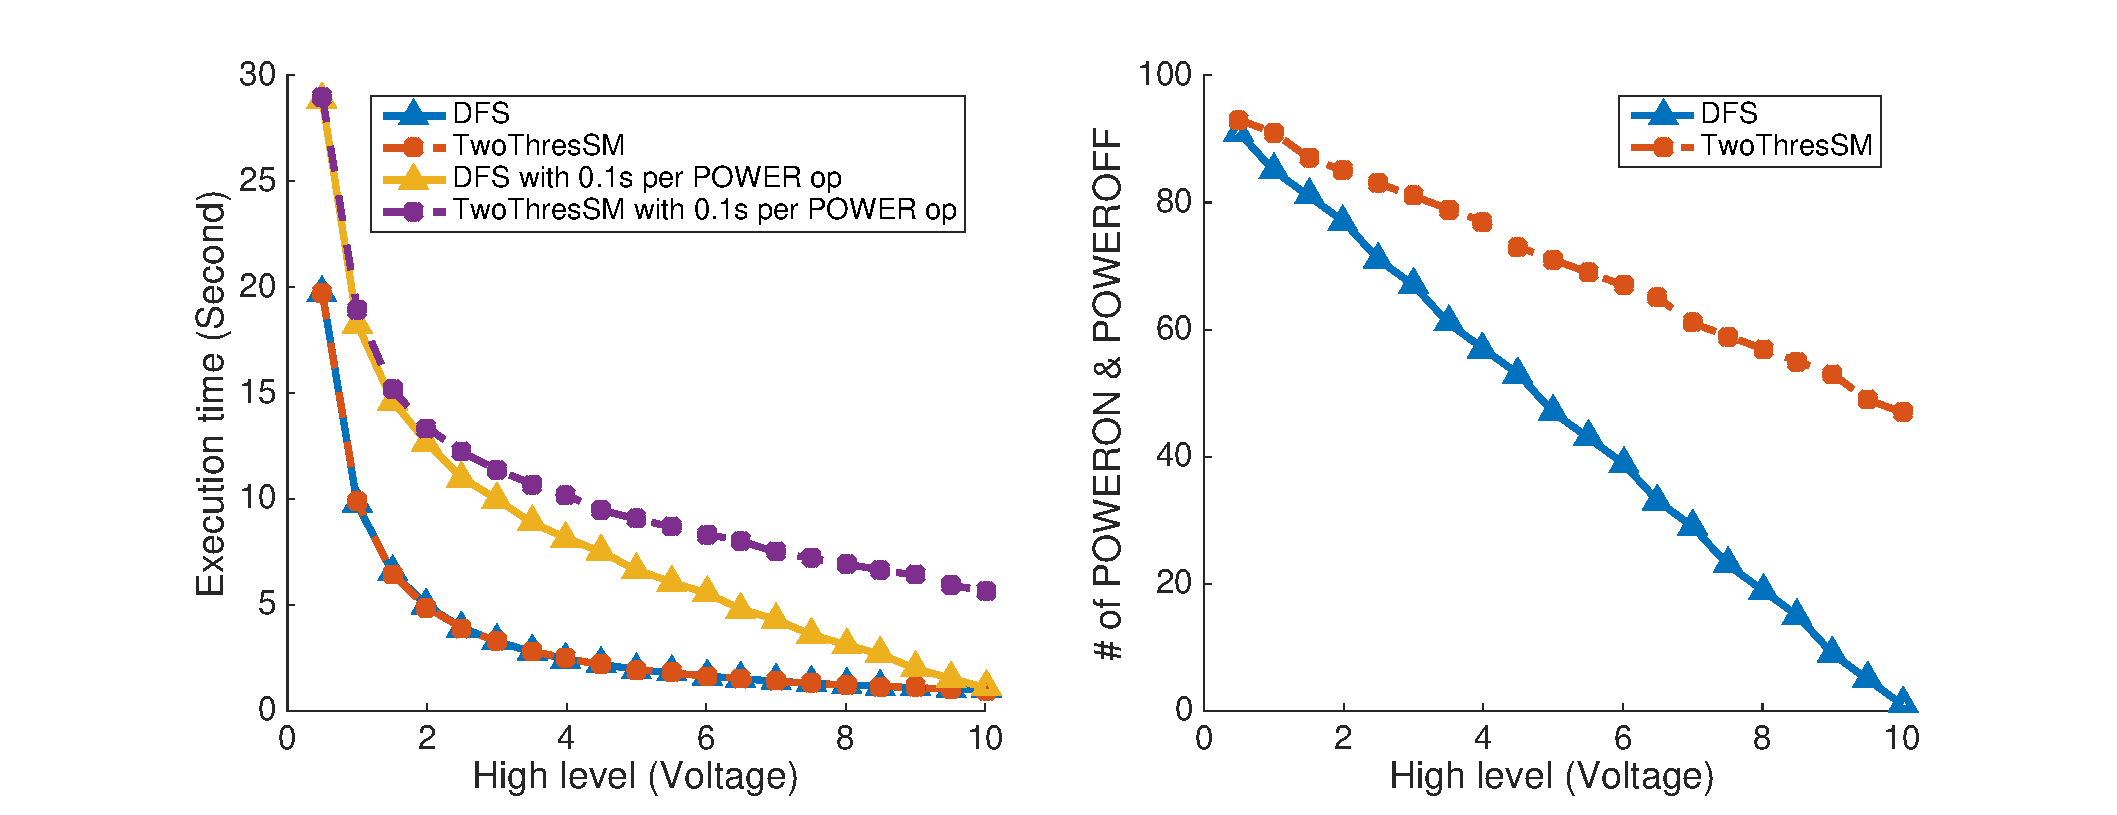
\includegraphics[width = 5.5in]{high.eps}
\caption{不同高电平下运行效率的比较,左图为执行时间、右图为程序执行过程中开关电源次数统计}
\label{high}
\end{figure}


\subsubsection{低电平}
接下来,我们对不同低电平(固定高电平为8V,占空比为50\%)的供能情况进行了分析,如图~\ref{low} 左下面两条曲线所示,DFS 与 TwoThresSM 都随着高电平的上升,系统性能越好,并且如果不考虑系统开关机的时间代价的话,两者的性能并没有太大的区别。

然而,根据我们的统计发现 (cf. 图~\ref{low} 右),TwoThresSM 相较于 DFS 在执行程序过程中所需要开关机的次数随着高电平的上涨差距越来越大,并且,DFS 在当前情况下,只需要低电平为 2V 左右即可使得系统几乎不断电持续工作,这对于系统的稳定性来说是至关重要的。
若考虑每次开机关机都需要0.1秒的时间,即可得到图~\ref{low} 左所示上面两条曲线,可以看到,两者性能有显著的差距。
\begin{figure}[!htbp]
\centering
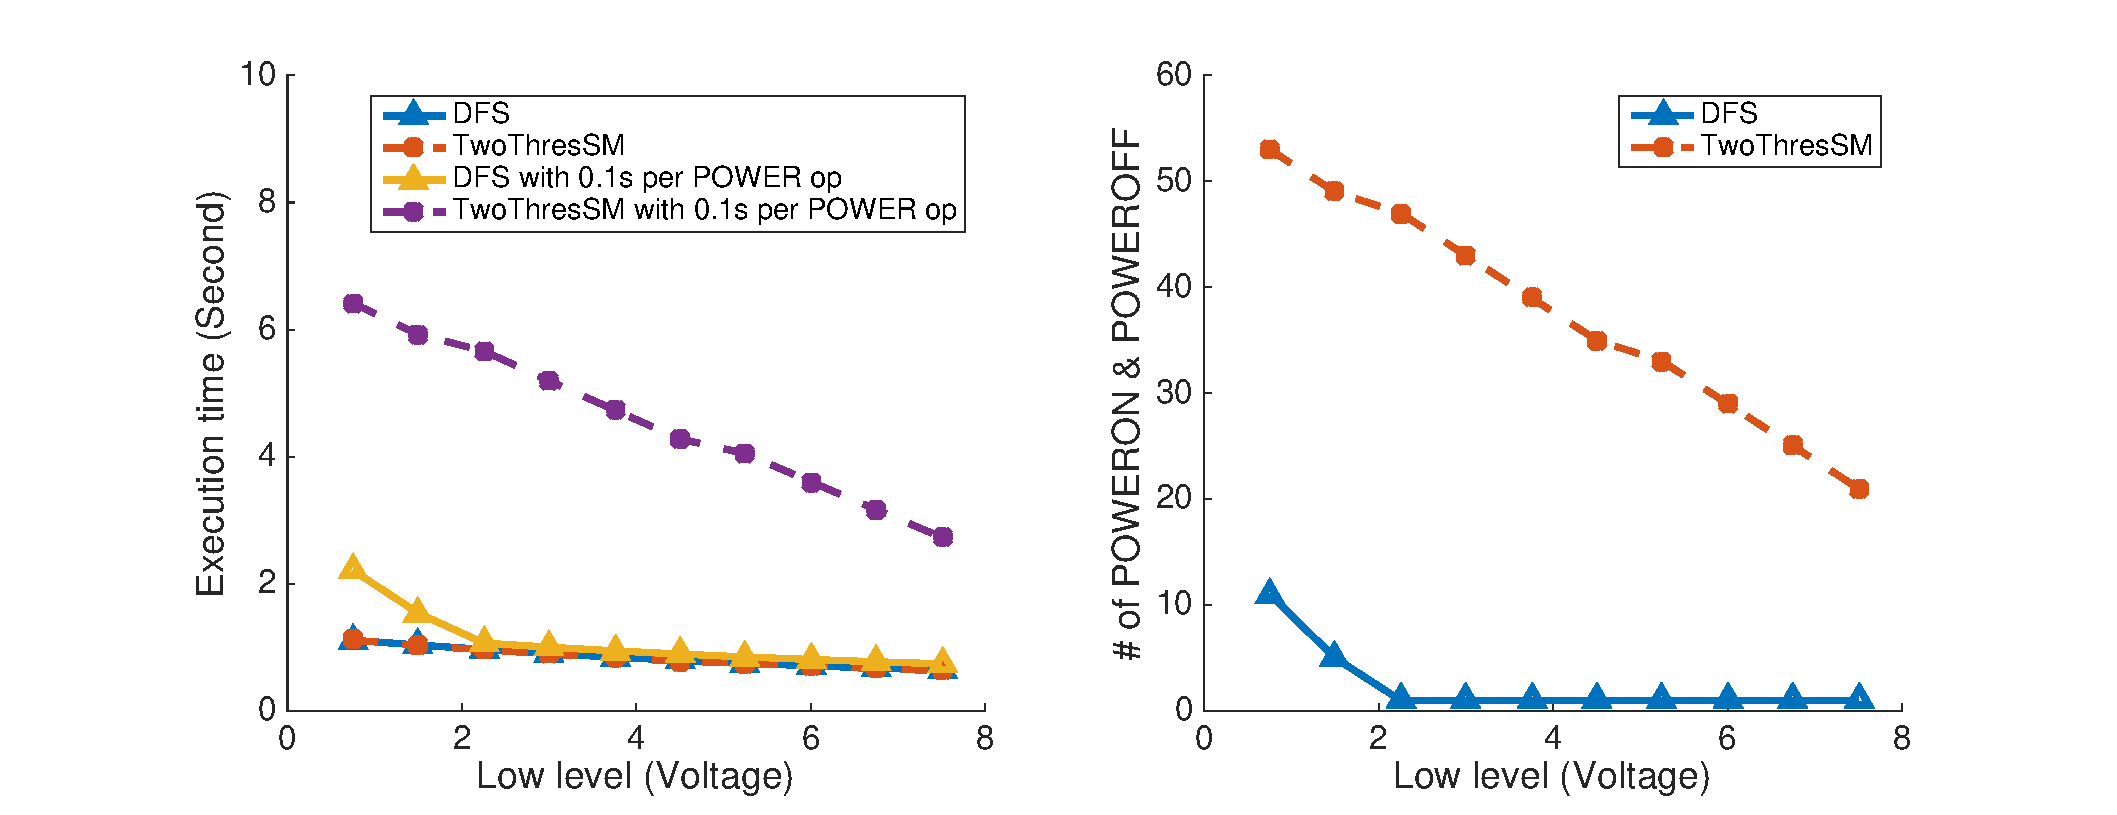
\includegraphics[width = 5.5in]{low.eps}
\caption{不同低电平下运行效率的比较,左图为执行时间、右图为程序执行过程中开关电源次数统计}
\label{low}
\end{figure}


\subsubsection{占空比}
接下来,我们对不同占空比(固定高电平为8V,低电平为3V)的供能情况进行了分析,如图~\ref{duty} 左下面两条曲线所示,DFS 与 TwoThresSM 都随着高电平的上升,系统性能越好,并且如果不考虑系统开关机的时间代价的话,两者的性能并没有太大的区别。

然而,根据我们的统计发现 (cf. 图~\ref{duty} 右),TwoThresSM 相较于 DFS 在执行程序过程中所需要开关机的次数随着高电平的上涨差距越来越大,并且,DFS 在当前情况下,只需要占空比为 0.4 左右即可使得系统十分稳定的持续工作。
若考虑每次开机关机都需要0.1秒的时间,即可得到图~\ref{duty} 左所示上面两条曲线,可以看到,两者性能有显著的差距。
\begin{figure}[!htbp]
\centering
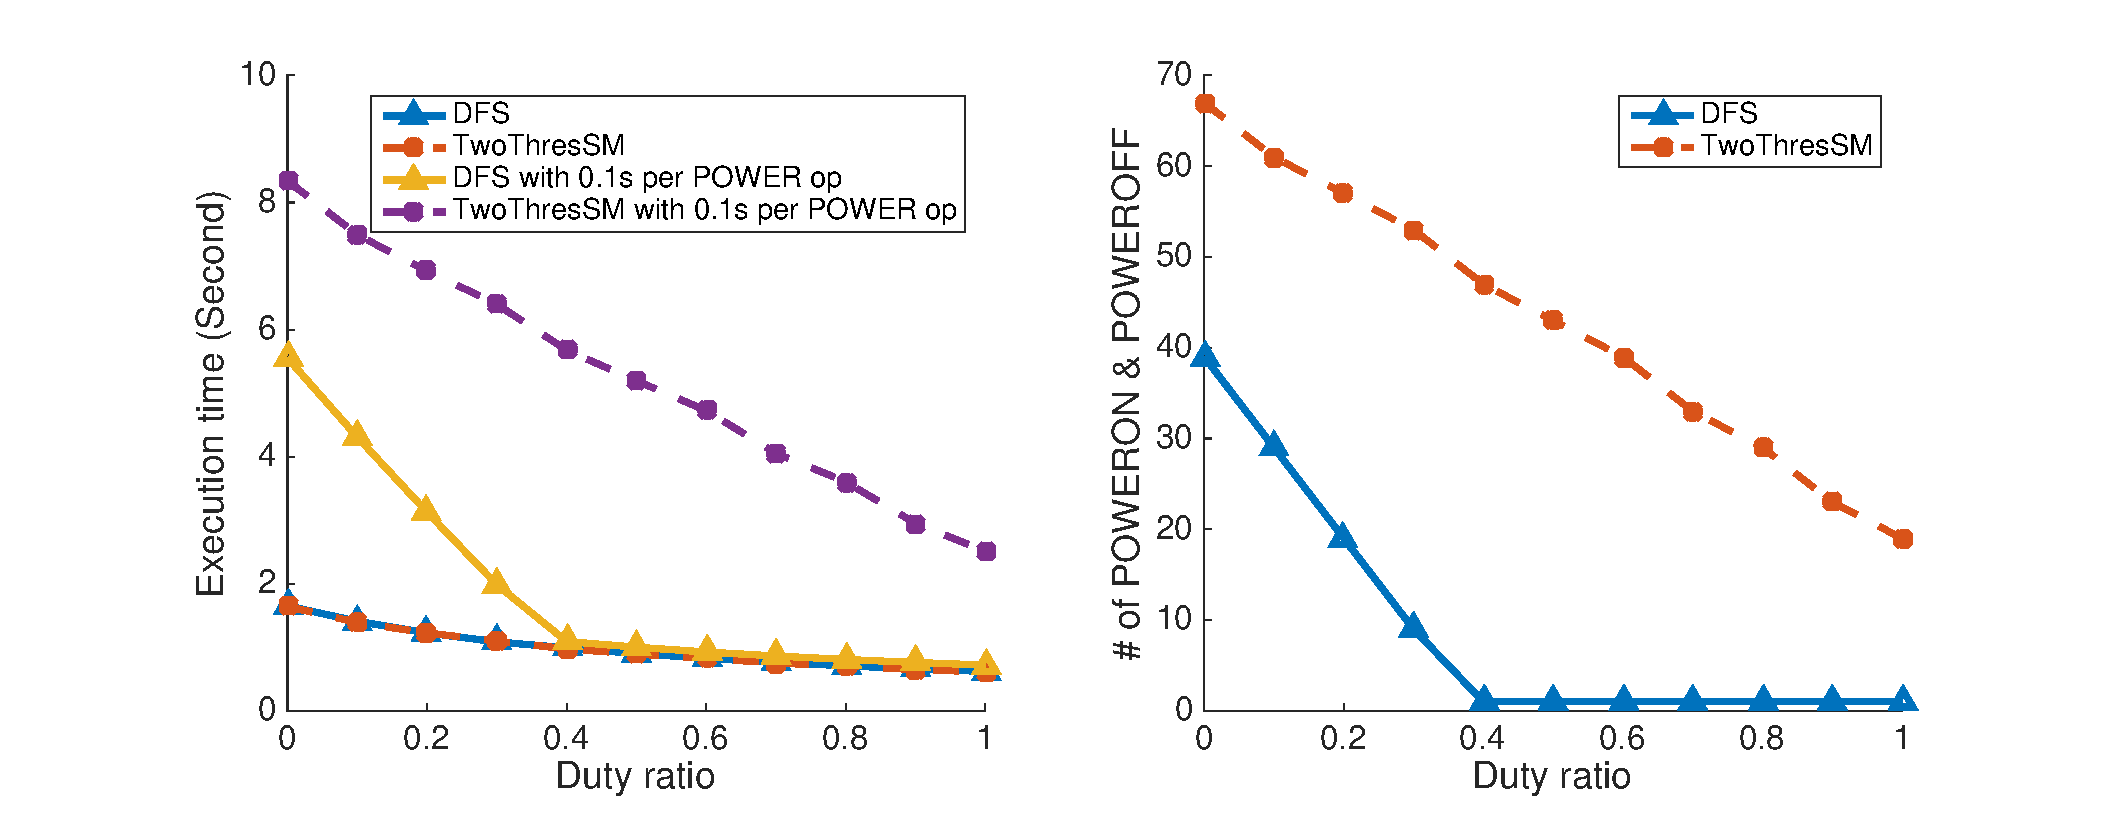
\includegraphics[width = 5.5in]{duty.eps}
\caption{不同占空比下运行效率的比较,左图为执行时间、右图为程序执行过程中开关电源次数统计}
\label{duty}
\end{figure}


\section{结论} \label{sec:conclusion}
本文对 gem5 以及 gem5-NVP 的关键结构做了一个系统性的整理以及介绍。同时,我们还在 gem5-NVP 的基础上搭建了一个 DFS 系统,并对不同能量环境的系统性能进行了仿真以及与原系统的比较,发现在稍微考虑开关机时间代价后,DFS 系统所带来的性能优化就十分可观。
未来我们希望引入开关机的能量代价以及切换频率的能量及时间代价,对 DFS 系统进行更全面的研究。

\bibliographystyle{plain}
\bibliography{hhh}

\end{document}
